\section{Digital Microfluidics (DMF)}
Digital microfluidics (DMF) represents a significant departure from traditional microfluidic techniques. Instead of relying on continuous flow through intricate channel geometries and external micropumps, DMF controls liquid movement by manipulating individual droplets on a planar surface using localized electric fields applied on an array of electrodes \cite{abdelgawadDigitalRevolutionNew2009,fairChemicalBiologicalApplications2007}.\\

Due to smaller form factor, DMF allows smaller liquid volume for laboratory processes to be in microliter (\textmugreek L) and picoliter (pL), thus reducing reagents and samples wastage \cite{bhattacharjeeDropletPositionControl2010,royNewSamplePreparation2015}.\\

Another advantage of DMF have over microfluidics are reduced sample cross-contamination and dispersion. This is due to the droplet served as a self-contained microreactor, there is negligible cross-mixing between different samples or reagents \cite{luoMachineVisionbasedDriving2021,wuResearchProgressElectrode2023}.\newpage

DMF are categorically divided into two configurations, which are open and closed as illustrated in Figure \ref{DMFConfig}.\\
\begin{figure}[h!]
    \centering
    \begin{subfigure}{0.45\textwidth}
        \centering
        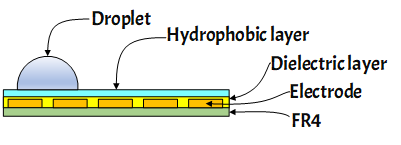
\includegraphics[width=\textwidth]{Open_TypeDMF.png}
        \caption{Open type DMF}
        \label{OpenTypeDMF}
    \end{subfigure}
    \begin{subfigure}{0.45\textwidth}
        \centering
        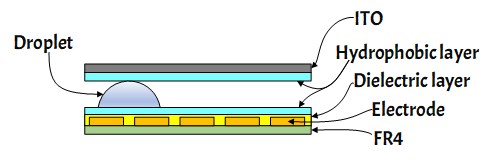
\includegraphics[width=\textwidth]{Closed_TypeDMF.png}
        \caption{Closed type DMF}
        \label{ClosedTypeDMF}
    \end{subfigure}
    \caption{Types of DMF configurations}
    \label{DMFConfig}
\end{figure}

Generally, key operations that can be executed by DMF are shown in Figure \ref{DMFOps} \cite{bhattacharjeeMultipleDilutionSample2012,bhattacharjeeEfficientGenerationDilution2019,bhattacharyaAlgorithmicChallengesDigital2014}. However, splitting and dispensing operations could not be achieved in open-configuration due to
\begin{figure}[h!]
    \smartdiagramset{bubble node font=\sffamily\large,
    bubble center node font=\sffamily\Huge}
    \centering
    \smartdiagram[bubble diagram]{
        DMF\\Operations,
        Transport,
        Merging,
        Splitting,
        Dispensing,
        Mixing,
        Storage,
        Sensing
        }
    \caption{DMF key operations}
    \label{DMFOps}
\end{figure}
